\documentclass[a4paper,11pt]{report}

% Paquetes de idioma y codificación
\usepackage[utf8]{inputenc}
\usepackage[T1]{fontenc}
\usepackage{graphicx}
\usepackage{hyperref}
\usepackage{amsmath, amssymb}
\usepackage[numbers]{natbib}
\usepackage{listings}
\usepackage{geometry}
\usepackage{float}
\usepackage{caption}
\usepackage{titlesec}
\titleformat{\chapter}[hang]{\normalfont\huge\bfseries}{\thechapter.}{1em}{}
\usepackage[utf8]{inputenc}
\setcounter{tocdepth}{3}



% Configuración de márgenes según las especificaciones
\geometry{
    top=1in,
    bottom=1in,
    left=1.25in,
    right=1.25in
}

% Fuente Arial 11pt
\renewcommand{\familydefault}{\sfdefault}

% Espaciado de línea de 1.5
\renewcommand{\baselinestretch}{1.5}

% Configurar numeración de páginas
\pagenumbering{arabic}

% Configuración de pies de figura y tablas
\captionsetup{
    font=small,
    labelfont=bf,
    justification=centering,
    singlelinecheck=false
}

\title{\textbf{Comparative Study of Delaunay Path Planner and RRT/RRT* for Path Planning in Autonomous Racing}}
\author{Rodrigo Carri\'on Caro}
\date{\today}

\begin{document}

\maketitle
\tableofcontents
\newpage

\chapter*{Glossary}
\addcontentsline{toc}{chapter}{Glossary}
\begin{itemize}
    \item \textbf{RRT} - Rapidly-Exploring Random Tree
    \item \textbf{ROS2} - Robot Operating System 2
    \item \textbf{Unity} - Motor de simulación
    \item \textbf{Path Planning} - Planificación de rutas
\end{itemize}
\newpage

\chapter*{Abstract}
\addcontentsline{toc}{chapter}{Abstract}
\section*{0.1 Contexto}
Escribe aquí el contexto del problema.

\section*{0.2 Objetivo}
Escribe aquí la descripción clara del propósito del proyecto.

\section*{0.3 Metodología}
Describe el enfoque de desarrollo y herramientas utilizadas.

\section*{0.4 Resultados principales}
Explica los principales hallazgos y comparación entre métodos.

\section*{0.5 Conclusión}
Menciona el impacto del estudio y posibles mejoras.
\newpage

\chapter*{Acknowledgements}
\addcontentsline{toc}{chapter}{Acknowledgements}

I would like to express my sincere gratitude to my supervisor, \textbf{Muhammad Younas}, for his guidance, support, and continuous feedback throughout this project. His insights were fundamental in shaping the structure and direction of the research.

My heartfelt thanks also go to the entire \textbf{Oxford Brookes Racing Autonomous (OBRA)} team for creating an environment of collaboration and technical excellence. In particular, I am especially grateful to \textbf{Aduén Benjumea} and \textbf{Mihir Gohad}, who served as project leads and played a crucial role in defining the vision and objectives of the team throughout the year.

I would also like to thank \textbf{Sebastian Donnelly}, whose deep experience within OBRA was invaluable—always available to solve doubts and provide practical advice during key stages of development. 

A special mention goes to \textbf{Dorian Amaritei}, who supported the development and optimization of the Delaunay path planner and contributed significantly to its refinement.

Finally, I am very thankful to \textbf{Pablo Gutiérrez}, lead of the simulation subteam, who assisted me in running and validating the simulations used to compare the planners. His help ensured that the performance of each algorithm could be observed under realistic and controlled scenarios.

This project would not have been possible without the collaborative effort and technical excellence of everyone involved.

\newpage


\chapter{Introduction}
\section{Background}

In autonomous vehicles, path planning is essential, as it allows for efficient and safe route
planning in real time. Specifically, the RRT algorithm \textquotedblleft RRT Rapidly exploring Random
Tree\textquotedblright can explore large spaces efficiently. This makes it ideal for dynamic environments,
such as an autonomous car race. These characteristics make it widely used in the field
of robotics. The RRT (Rapidly exploring Random Tree) algorithm is a search method
used to efficiently find paths in large spaces \cite{reference1}. It is particularly useful in dynamic
environments where viable paths need to be found quickly in real-time. Currently, the
Oxford Brookes Racing Autonomous (OBRA) team uses a neural network path planner.
A Delaunay path planner is being developed but has not yet been implemented. These
approaches present some limitations in real-time situations. The development and implementation of an RRT \cite{reference2} will allow for greater flexibility and adaptability. Ideally, this
will improve the team’s path planning capabilities. In addition to developing the RRT,
this project will compare its performance with the current Delaunay path planner. By
evaluating their efficiency and adaptability in dynamic scenarios, the goal is to determine
which algorithm provides better results for autonomous racing.

\section{Aim}
The aim of this project is to develop and optimize two advanced path planning algorithms for autonomous racing: an improved Delaunay-based planner and an optimized RRT* algorithm. These planners will be designed to enhance adaptability, computational efficiency, and trajectory optimization in high-speed, dynamic environments. 

This project also aims to conduct a detailed comparative analysis of both algorithms, evaluating their performance across key metrics such as computation time, path efficiency, adaptability to dynamic obstacles, and robustness under racing conditions. 

By implementing and testing these algorithms within a ROS2-based simulation environment using Unity, this research seeks to identify the most effective path planning solution for the OBRA team's autonomous racing vehicle. The insights gained from this study will contribute to both the OBRA competition strategy and the broader field of autonomous vehicle navigation.


\section{Objectives}
\begin{itemize}
    \item To conduct a comprehensive study of path planning techniques used in autonomous vehicle navigation, analyzing their advantages, limitations, and applications in high-speed racing scenarios. \cite{reference3}
    \item To develop and implement an improved Delaunay-based path planner that enhances adaptability, computational efficiency, and trajectory smoothness in dynamic environments.
    \item To develop and implement an RRT algorithm from scratch for real-time path planning in autonomous vehicles, ensuring compatibility with the OBRA car's ROS2 framework.
    \item To optimize the RRT algorithm by integrating RRT* \cite{reference4}, improving its ability to generate efficient and dynamically adaptable routes.
    \item To validate both the optimized Delaunay and RRT* algorithms in a controlled simulation environment using Unity, testing their performance under varying racing conditions.
    \item To conduct a detailed comparative analysis of the optimized Delaunay and RRT* algorithms, evaluating key performance metrics such as computation time, path efficiency, adaptability to dynamic obstacles, and robustness in high-speed scenarios.
    \item To identify and address potential limitations of each algorithm, proposing refinements or hybrid approaches that could further enhance their performance.
    \item To integrate the most effective path planner into the OBRA team's autonomous racing pipeline, ensuring real-world applicability and alignment with competition requirements.
\end{itemize}


\section{Product Overview}
\subsection{Scope}
The objective of this project is to develop and optimize two new path planners for autonomous racing:
\begin{itemize}
    \item Optimized Delaunay Path Planner – A modified version of the traditional Delaunay-based planner, improving its efficiency and adaptability for dynamic racing environments.
    \item RRT* – An enhanced Rapidly-exploring Random Tree algorithm that generates smoother and more efficient paths by reducing randomness and refining route selection.
\end{itemize}
Both planners will be developed in Python, ensuring seamless integration with the ROS2 framework used in the OBRA autonomous car. The testing and validation process will be conducted in simulation environments using Unity, allowing for extensive evaluation before potential real-world implementation.
Once developed, these two new planners will be compared to determine which provides better performance in terms of adaptability, computational efficiency, and trajectory smoothness under high-speed, dynamic conditions.

\subsection{Audience}
The primary audience for this study is the Oxford Brookes Racing Autonomous (OBRA) team, as the improved path planning algorithms will directly contribute to their autonomous racing performance.
Additionally, this research is relevant to the academic community, particularly in robotics, AI, and autonomous vehicle navigation, by providing insights into optimization strategies for real-time path planning.
From an industry perspective, this study holds significance for autonomous systems professionals, particularly those developing path planning solutions for high-speed and dynamic environments, such as self-driving vehicles, robotics, and UAV navigation.


\newpage

\chapter{Background Review}
\section{Related Literature}

\begin{table}[H]
    \centering
    \begin{tabular}{|p{3cm}|p{10cm}|}
        \hline
        \textbf{Reference} & Zhao, H., Wu, Z., Li, Y., \& Wang, J. (2021) ‘Improved Bidirectional RRT* Path Planning Method for Smart Vehicle’, Mathematical Problems in Engineering, pp. 1-14. doi: 10.1155/2021/6669728. \\ \hline
        \textbf{Title} & Improved Bidirectional RRT* Path Planning Method for Smart Vehicle \\ \hline
        \textbf{Summary} & The study proposes an improvement to the bidirectional RRT* algorithm to optimize route planning in intelligent vehicles, aiming for shorter and more efficient routes. \\ \hline
        \textbf{Evaluation} & The approach is useful for static environments, but it does not sufficiently address the challenges in dynamic environments, which may limit its applicability in competitive vehicles. \\ \hline
        \textbf{Reflection} & The proposed improvements could be applied to optimize the RRT* algorithm in my project, particularly in reducing computation time and optimizing routes. \\ \hline
        \textbf{Main Themes} & RRT* optimization, route planning, autonomous vehicles. \\ \hline
    \end{tabular}
    \caption{Summary of Zhao et al. (2021)}
    \label{tab:zhao2021}
\end{table}

\begin{table}[H]
    \centering
    \begin{tabular}{|p{3cm}|p{10cm}|}
        \hline
        \textbf{Reference} & Gasparetto, A., Boscariol, P., Lanzutti, A., \& Vidoni, R. (2015) ‘Path Planning and Trajectory Planning Algorithms: A General Overview’, Journal of Intelligent \& Robotic Systems, pp. 1-33. doi: 10.1007/978-3-319-14705-5\_1. \\ \hline
        \textbf{Title} & Path Planning and Trajectory Planning Algorithms: A General Overview \\ \hline
        \textbf{Summary} & The article provides an overview of the main trajectory and route planning algorithms in robotics. It analyses methods such as Roadmap, Cell Decomposition, and RRT, as well as their applications in industrial and autonomous environments. \\ \hline
        \textbf{Evaluation} & The study offers a comprehensive overview of the algorithms but focuses more on static industrial systems, limiting its applicability to dynamic environments. However, the review of RRT is useful for improving my project. \\ \hline
        \textbf{Reflection} & This article will be key to contextualizing my work, as it provides a solid foundation on traditional methods and suggests possible areas for improvement, such as applying them in more dynamic environments. \\ \hline
        \textbf{Main Themes} & Route planning, RRT, optimization algorithms, autonomous robotics. \\ \hline
    \end{tabular}
    \caption{Summary of Gasparetto et al. (2015)}
    \label{tab:gasparetto2015}
\end{table}

\begin{table}[H]
    \centering
    \begin{tabular}{|p{3cm}|p{10cm}|}
        \hline
        \textbf{Reference} & Wang, H., Li, G., Hou, J., Chen, L., \& Hu, N. (2022) ‘A Path Planning Method for Underground Intelligent Vehicles Based on an Improved RRT* Algorithm,’ Electronics, vol. 11, no. 3, p. 294. doi: 10.3390/electronics11030294. \\ \hline
        \textbf{Title} & A Path Planning Method for Underground Intelligent Vehicles Based on an Improved RRT* Algorithm \\ \hline
        \textbf{Summary} & The study proposes an improved RRT* method for route planning in underground intelligent vehicles, adjusting the dynamic step size and turn angle constraints. \\ \hline
        \textbf{Evaluation} & The approach is innovative for underground environments and offers improvements in efficiency and safety, but it is limited to controlled spaces and does not address navigation in fully dynamic environments. \\ \hline
        \textbf{Reflection} & This study is relevant to my project, as the proposed RRT* improvements could be applied to optimize the algorithm in more complex scenarios, such as autonomous racing. \\ \hline
        \textbf{Main Themes} & RRT*, underground autonomous vehicles, route planning, optimization. \\ \hline
    \end{tabular}
    \caption{Summary of Wang et al. (2022)}
    \label{tab:wang2022}
\end{table}

\begin{table}[H]
    \centering
    \begin{tabular}{|p{3cm}|p{10cm}|}
        \hline
        \textbf{Reference} & Sánchez-Ibáñez, J.R., Pérez-del-Pulgar, C.J., \& García-Cerezo, A. (2021) ‘Path Planning for Autonomous Mobile Robots: A Review’, Sensors 2021, 21, 7898. doi: 10.3390/s21237898. \\ \hline
        \textbf{Title} & Path Planning for Autonomous Mobile Robots: A Review. \\ \hline
        \textbf{Summary} & The article reviews route planning algorithms for mobile robots, focusing on their classification and applicability in autonomous environments. \\ \hline
        \textbf{Evaluation} & It provides a very useful overview of the main approaches, but it focuses on controlled scenarios and may be limited for dynamic environments such as competitions. \\ \hline
        \textbf{Reflection} & This article provides a good foundation for comparing different approaches, which will help me justify the choice of RRT in my project. \\ \hline
        \textbf{Main Themes} & Route planning, mobile robots, path search algorithms. \\ \hline
    \end{tabular}
    \caption{Summary of Sánchez-Ibáñez et al. (2021)}
    \label{tab:sanchez2021}
\end{table}

\begin{table}[H]
    \centering
    \begin{tabular}{|p{3cm}|p{10cm}|}
        \hline
        \textbf{Reference} & C. Messer, A. T. Mathew, N. Mladenovic and F. Renda, "CTR DaPP: A Python Application for Design and Path Planning of Variable-strain Concentric Tube Robots," 2022 IEEE 5th International Conference on Soft Robotics (RoboSoft), Edinburgh, United Kingdom, 2022, pp. 14-20, doi: 10.1109/RoboSoft54090.2022.9762088. \\ \hline
        \textbf{Title} & CTR DaPP: A Python Application for Design and Path Planning of Variable-strain Concentric Tube Robots. \\ \hline
        \textbf{Summary} & The study presents a modular platform in Python that uses the RRT* algorithm for route planning and design optimization in concentric tube robots. It focuses on trajectory planning in environments with torsion and curvature constraints. \\ \hline
        \textbf{Evaluation} & The implementation in Python is relevant to my project, as it allows for the flexible use of planning and optimization algorithms. \\ \hline
        \textbf{Reflection} & This article supports the use of Python in my project, demonstrating that it is an effective option for developing and testing algorithms like RRT*. \\ \hline
        \textbf{Main Themes} & RRT*, route planning, concentric tube robots, design optimization, use of Python. \\ \hline
    \end{tabular}
    \caption{Summary of Messer et al. (2022)}
    \label{tab:messer2022}
\end{table}

\begin{table}[H]
    \centering
    \begin{tabular}{|p{3cm}|p{10cm}|}
        \hline
        \textbf{Reference} & Kolski, S., Ferguson, D., Stachniss, C., \& Siegwart, R. (2006) 'Autonomous Driving in Dynamic Environments', Proceedings of the 2006 IEEE/RSJ International Conference on Intelligent Robots and Systems, pp. 1-10. doi: 10.3929/ethz-a-010079481. \\ \hline
        \textbf{Title} & Autonomous Driving in Dynamic Environments. \\ \hline
        \textbf{Summary} & The study presents a hybrid autonomous navigation system that operates in both structured and unstructured environments, handling dynamic obstacles like pedestrians and other vehicles. \\ \hline
        \textbf{Evaluation} & Unlike many approaches focused on static environments, this system is highly relevant for dynamic settings, such as autonomous car competitions, where real-time adjustments to moving obstacles are critical. \\ \hline
        \textbf{Reflection} & This study is essential for my project as it highlights the importance of dynamic environments and provides useful insights for improving my route planning system. \\ \hline
        \textbf{Main Themes} & Autonomous navigation, dynamic environments, route planning, moving obstacles, autonomous vehicles. \\ \hline
    \end{tabular}
    \caption{Summary of Kolski et al. (2006)}
    \label{tab:kolski2006}
\end{table}

\chapter{Methodology}
\section{Research and Software Development Process}

\subsection{Application of Agile Methodology, aqui meto el diagrama de Agile}
The project follows an Agile methodology, allowing for iterative progress and continuous refinement of the algorithms. This approach ensures flexibility and adaptability to changing requirements. Agile was chosen over traditional models such as Waterfall, as the latter requires a rigid, sequential structure that does not accommodate modifications once development begins.

Given the dynamic nature of this project, the Agile framework supports the parallel development of:
\begin{itemize}
    \item Optimization and rewriting of the existing \textbf{Delaunay path planner}.
    \item Development of a new \textbf{RRT* algorithm} from scratch.
    \item Comparative testing and analysis of both approaches.
\end{itemize}

The project is structured into multiple iterations, ensuring continuous validation and improvement of the implemented methods.

\section{Development Phases}
The preparation phase involved selecting the topic and conducting meetings with OBRA to align the project's objectives. A proposal was submitted and refined based on feedback, followed by setting up the required system and environment, including Unity and ROS2. An initial progress report was submitted to document early findings, and research was conducted to establish a baseline for optimising the Delaunay path planner.

The first iteration focused on enhancing the Delaunay-based path planner by rewriting the algorithm to improve its efficiency and adaptability. An optimised version was implemented and tested in a simulation environment to validate improvements in path generation. The results were then demonstrated before proceeding with the development of the RRT algorithm.

In the second iteration, work began on the RRT algorithm by conducting a theoretical study to understand its principles and limitations. This was followed by research and design for a basic implementation, which was then developed and tested in a simulated environment to compare its performance with the Delaunay approach.

Once the basic RRT implementation was completed, the third iteration concentrated on optimising it using RRT*. This involved refining the algorithm to enhance route efficiency and conducting a comparative analysis between Delaunay and RRT* under racing conditions to assess their performance.

Following the comparative tests, the project progressed to the final validation and integration phase. The selected algorithm was integrated into the OBRA car to ensure its applicability in real-world racing scenarios.

The final stage of the project involved preparing a comprehensive report summarising the findings, results, and technical contributions. Additionally, a final presentation was developed to communicate the project's outcomes and submit the final deliverables.




\chapter{Technology}
\section{Implementation Tools and Resources}
The development of this project relies on several key technologies and tools to ensure efficient implementation and testing. The primary programming language used is Python, which serves as the backbone of the implementation. Python is used to develop the path-planning algorithms, integrate them into ROS2, and manage the necessary data processing tasks. Its extensive libraries and compatibility with machine learning and robotic frameworks make it ideal for rapid prototyping and testing.

For robotic integration, we utilize ROS2 (Humble), which facilitates seamless communication between different components of the autonomous system. ROS2 manages sensor data processing, real-time control, and path planning, ensuring that all modules operate in a synchronized manner. The middleware's efficiency in handling multiple nodes is crucial for real-time decision-making within the autonomous vehicle.

The project runs on Ubuntu 22.04, which provides a stable and well-supported environment for ROS2, Python-based applications, and simulation tools. Ubuntu ensures compatibility with the robotic frameworks used in this project and offers an extensive community for troubleshooting and optimization.

For version control, Git and GitLab serve as the central repository for managing code changes. The OBRA workspace on GitLab stores previous developments and is used to track new implementations through branches. Frequent commits help maintain a structured development workflow.

Simulation and testing are conducted using a structured environment that combines Unity for scenario modeling and Foxglove for real-time visualization of vehicle states and planned paths. The simulation outputs, along with test results, are stored in Google Drive, ensuring efficient data management and accessibility for analysis.

To maintain an organized workflow, Notion is used for task management and Agile planning, ensuring that development is well-structured and efficiently executed.

By integrating these technologies, we aim to develop a robust and scalable path-planning solution that seamlessly integrates with the OBRA autonomous vehicle.

\section{Workspace}

To visualize the structure of the OBRA ecosystem, we can execute the following command in the Ubuntu terminal:

\begin{verbatim}
rqt_graph
\end{verbatim}

This command generates a graphical representation of the ROS2 nodes and topics in execution. To obtain a visualization similar to the one shown in Figure \ref{fig:obra_graph}, it is necessary to have the simulator and the workspace running and properly configured.

\begin{figure}[h]
    \centering
    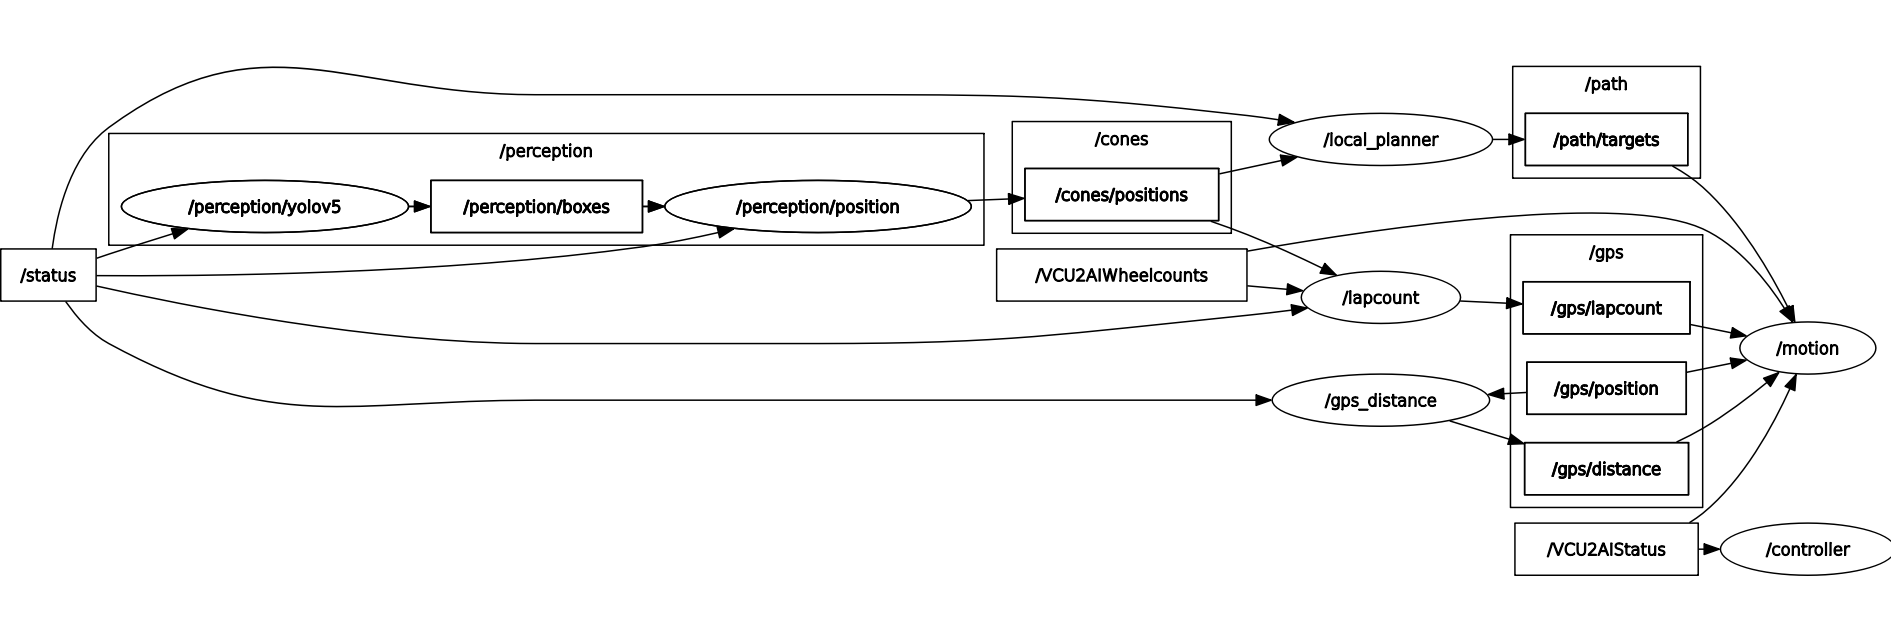
\includegraphics[width=\textwidth]{Images/wsgraph.png}
    \caption{Ecosystem of nodes and topics in OBRA generated with rqt\_graph}
    \label{fig:obra_graph}
\end{figure}

The OBRA workspace consists of multiple nodes that interact through ROS2 topics, enabling communication between different modules of the autonomous system. In the graph generated by \texttt{rqt\_graph}, we can observe how the different components are organized and communicate.

The \texttt{/status} node provides system information and connects with other key modules. Within the perception subsystem, the \texttt{/perception/yolov5} node processes images and generates bounding boxes, which are sent to \texttt{/perception/boxes} and subsequently converted into positions through \texttt{/perception/position}. This information is used by other modules such as path planning and localization.

The cone detection module processes position data through the \texttt{/cones/positions} topic, integrating this data into route planning via \texttt{/local\_planner} and lap counting via \texttt{/lapcount}. Additionally, the GPS module handles localization data through \texttt{/gps/lapcount}, \texttt{/gps/position}, and \texttt{/gps/distance}, providing essential information for autonomous navigation.

Finally, the control module processes all this information and transmits it to \texttt{/motion}, enabling movement execution in the autonomous vehicle. The communication between these modules ensures the proper operation of the system in a simulation environment or in the real vehicle.

The following subsections describe the various system modules in detail:

\subsection{Cones}

\subsection{Perception}

\subsection{Localization \& Mapping}

\subsection{Path Planning}

\subsection{Control}




\section{Simulation and Testing Tools}

The simulation and testing phase plays a crucial role in validating the path-planning algorithms before deployment in the real OBRA autonomous vehicle. The core of the simulation environment is built using Unity, which provides a controlled and highly customizable setting where different track conditions, obstacles, and environmental variations can be modeled. Unity allows us to evaluate the performance of the algorithms under high-speed driving scenarios, tight turns, and unexpected obstacles, ensuring that the vehicle can navigate efficiently and safely.

To complement the simulation process, we use Foxglove for real-time visualization and analysis of key system data. Since our project is built on ROS2 (Humble), Foxglove acts as an interface to monitor ROS2 topics, displaying critical information such as vehicle state, planned trajectories, sensor readings, and dynamic obstacle detection. This visualization is essential for debugging, performance assessment, and fine-tuning the parameters of our path-planning algorithms.

The validation process is structured around a set of performance metrics, ensuring that each algorithm is assessed based on objective criteria. These metrics include:
\begin{itemize}
    \item Path efficiency: Measuring the distance and curvature of the generated trajectory.
    \item Computational speed: Evaluating how quickly the algorithm produces a valid path.
    \item Adaptability to dynamic environments: Testing how well the planner reacts to changes such as moving obstacles or shifting track conditions.
\end{itemize}

Once the simulations are completed, the results, including logs, performance data, and video recordings, are stored in Google Drive for further analysis and comparison. This repository allows the team to track improvements over time and make data-driven decisions when optimizing the algorithms.

By integrating Unity for simulation, Foxglove for real-time monitoring, and Google Drive for data storage, we establish a structured and efficient testing framework. This ensures that our path-planning algorithms are rigorously validated before integration into the OBRA vehicle, minimizing risks and maximizing system reliability.





\chapter{Code Development}

\section{Path Planning Folder Structure}

To understand the overall structure of the path planning folder, we can refer to the diagram in Figure \ref{fig:path_planning_structure}. This structure organises different components responsible for planning the vehicle's path using either the Delaunay triangulation method or the RRT* algorithm.

\begin{figure}[h]
    \centering
    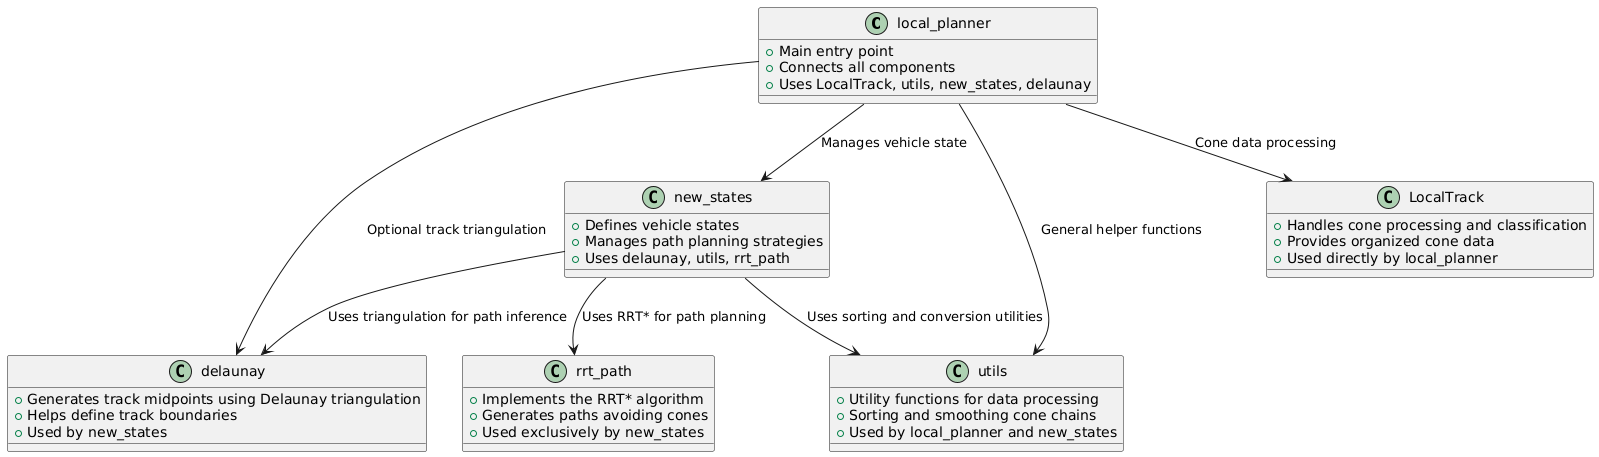
\includegraphics[width=\textwidth]{Images/local_planner.png}
    \caption{Path planning folder structure}
    \label{fig:path_planning_structure}
\end{figure}

The main entry point of the path planning system is the \texttt{local\_planner.py} script. This module connects all components and manages the overall planning process. Within \texttt{local\_planner}, the function \texttt{change\_state(self)} determines whether to use Delaunay or RRT* based on the detected environment. The selection is made using the following lines of code:

\begin{verbatim}
self.state = RRTStarState(self)  # Uses RRT* for path planning
self.state = Delaunay(self)      # Uses Delaunay for path inference
\end{verbatim}

\subsection{Local Planner (local\_planner.py)}
The \texttt{local\_planner.py} script serves as the core component of the path planning system. It is responsible for subscribing to relevant ROS2 topics, processing incoming data, and determining the appropriate path planning algorithm. The script maintains real-time vehicle position updates and cone detection to adjust its planning method dynamically.

A key function in \texttt{local\_planner.py} is \texttt{change\_state(self)}, which decides whether to use the RRT* or Delaunay algorithm based on the available cone data:

\begin{verbatim}
def change_state(self):
    """
    Determines the path planning method based on detected cones.
    """
    if count_blue > 0 and count_yellow > 0 and count_blue + count_yellow > 2:
        self.state = RRTStarState(self)  # Selects RRT* for complex scenarios
    else:
        self.state = Delaunay(self)  # Defaults to Delaunay triangulation
\end{verbatim}

The function first verifies if the system has detected both blue and yellow cones. If a sufficient number of cones are present, it selects \texttt{RRTStarState}, as the RRT* algorithm is better suited for handling complex, dynamic paths. If fewer cones are detected, it defaults to Delaunay triangulation, which relies on precomputed track midpoints for a stable and structured path.

\subsection{State Management (new\_states.py)}
The \texttt{new\_states.py} module defines the behaviour of different path planning strategies. It manages vehicle states and allows seamless switching between planning methods depending on the track conditions. The state management system is based on an abstract class \texttt{LocalPlannerState}, which enforces the implementation of a \texttt{plan\_path} method in all subclasses.

One of the primary states is \texttt{RRTStarState}, which utilises the RRT* algorithm for adaptive path generation:

\begin{verbatim}
class RRTStarState(LocalPlannerState):
    def plan_path(self):
        """Implements the RRT* algorithm for path planning."""
        try:
            # Ensure car position is defined
            if not hasattr(self.context, "car_position") or self.context.car_position is None:
                print("Warning: `car_position` is not defined.")
                return self.context.last_path

            # Extract cone positions from the local track
            cones_blue = cones_to_tuple_list(self.context.local_track.blue)
            cones_yellow = cones_to_tuple_list(self.context.local_track.yellow)
            
            # Instantiate the RRT* planner
            rrt_planner = RRTStarPlanner(cones_blue, cones_yellow)
            
            # Generate the path using RRT*
            path = rrt_planner.plan_path(start=self.context.car_position, goal=self.context.target_position)
            
            if path is None:
                print("Warning: RRT* did not find a path, using last known path.")
                return self.context.last_path

            return path
        except Exception as e:
            print(f"Warning: RRT* encountered an error: {e}")
            return self.context.last_path
\end{verbatim}

This function first ensures that the car's position is known. It then extracts cone locations and passes them to the \texttt{RRTStarPlanner}, which attempts to compute an optimal path. If the planner fails, it defaults to the last successful path to maintain stability.

\subsection{Utility Functions (utils.py)}
The \texttt{utils.py} module provides helper functions for sorting cone data, smoothing paths, and handling data conversions.

\begin{verbatim}
def sort_cone_chain(cones):
    """Sorts cones into a continuous chain for path planning."""
    return sorted(cones, key=lambda c: c.x)
\end{verbatim}

By integrating these components, the path planning system dynamically selects the best algorithm for any given scenario, ensuring optimal performance in autonomous racing conditions.


\section{Initial Path Planner: Old Delaunay Implementation}
The initial path planner used by the OBRA autonomous vehicle during FSUK 2024 was based on the Delaunay triangulation method. This path planner was developed by the team throughout 2023 and 2024 and served as the foundation for autonomous navigation in the competition. The system relied on the detection of blue and yellow cones to generate a track boundary and compute a smooth path through the midpoints of the triangulated structure. By leveraging Delaunay triangulation, the planner provided a stable and predictable route, ensuring the vehicle could navigate efficiently. The initial Delaunay-based path planner lacks adaptability in dynamic environments, as it relies on static triangulation of detected cones. It struggles with inconsistent cone placement, cannot handle sudden obstacles efficiently, and lacks path smoothing, leading to suboptimal trajectories. Additionally, it does not optimise paths for minimal turns or distance.This implementation, while effective, had limitations in dynamic obstacle avoidance and adaptability, leading to further refinements in subsequent iterations.

\section{Delaunay Path Planner Optimization and Rewriting}

The optimization of the Delaunay path planner resulted in a significant reduction in complexity, improving both efficiency and maintainability. The previous implementation contained over 750 lines of code, relying on a complex graph-based approach to manage cone connections and extract midpoints. The new implementation, reduced to under 200 lines, introduces a streamlined structure based on the \texttt{TrackNavMesh} class, which efficiently handles the Delaunay triangulation and simplifies the extraction of midpoints.

\begin{figure}[h]
    \centering
    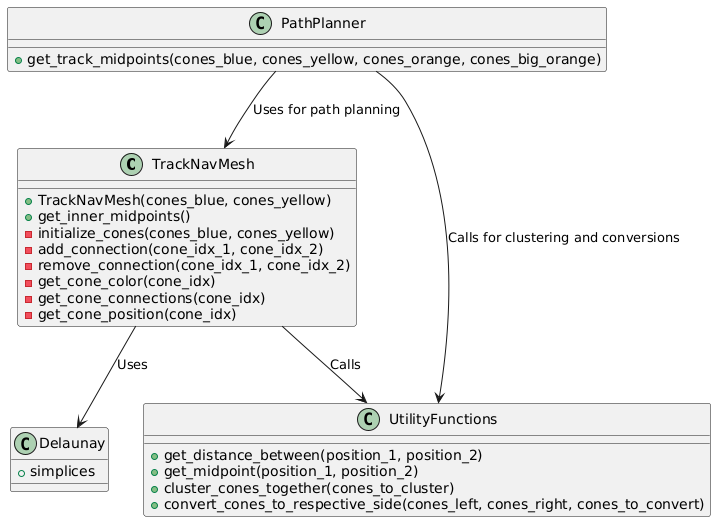
\includegraphics[width=\textwidth]{Images/delaunay.png}
    \caption{Optimized Delaunay Path Planning System}
    \label{fig:delaunay_optimization}
\end{figure}

Figure \ref{fig:delaunay_optimization} illustrates the restructured Delaunay path planner, highlighting key components and their interactions. The new system is structured around four main elements: \texttt{PathPlanner}, \texttt{TrackNavMesh}, \texttt{Delaunay}, and \texttt{UtilityFunctions}.

\subsection{Structural Simplification}
Previously, the planner relied on a manually managed graph structure to connect cones and determine midpoints. The new approach abstracts these operations into \texttt{TrackNavMesh}, which directly utilizes the \texttt{Delaunay} class from SciPy to establish relationships between cones.

\begin{verbatim}
def get_inner_midpoints(self):
    result = []
    for triangle in self.delaunay.simplices:
        for cone_idx in triangle:
            for other_cone_idx in triangle:
                if self.get_cone_color(cone_idx) != self.get_cone_color(other_cone_idx):
                    self.add_connection(cone_idx, other_cone_idx)
\end{verbatim}

By leveraging Delaunay triangulation directly, the system no longer requires redundant connection management, reducing computational overhead.

\subsection{Efficient Midpoint Calculation}
In the previous version, midpoint calculations involved multiple nested loops and redundant filtering. The optimized implementation directly extracts necessary midpoints from the triangulation and computes distances efficiently:

\begin{verbatim}
def get_distance_between(position_1, position_2):
    return math.hypot(position_1[0] - position_2[0], position_1[1] - position_2[1])
\end{verbatim}

This approach consolidates distance calculations into a single function, removing unnecessary recalculations.

\subsection{Enhanced Cone Clustering for Smoother Paths}
The old system inconsistently merged closely positioned cones, sometimes leading to erratic paths. The new implementation introduces \texttt{cluster\_cones\_together}, which ensures cones within a threshold distance are merged systematically.

\begin{verbatim}
def cluster_cones_together(cones_to_cluster):
    any_cone_within_max_cluster_distance = True
    while any_cone_within_max_cluster_distance:
        any_cone_within_max_cluster_distance = False
        for cone in cones_to_cluster:
            for next_cone in cones_to_cluster:
                if cone == next_cone: continue
                if get_distance_between(cone, next_cone) < MAX_CLUSTER_DISTANCE:
                    cones_to_cluster.append(get_midpoint(cone, next_cone))
                    cones_to_cluster.remove(cone)
                    cones_to_cluster.remove(next_cone)
                    any_cone_within_max_cluster_distance = True
\end{verbatim}

This method ensures smooth trajectories by preventing unnecessary sharp turns in the generated paths.

\subsection{Comparison of Old vs. New Implementation}
The table below highlights key improvements in the optimized Delaunay path planner:

\begin{table}[h]
    \centering
    \resizebox{\textwidth}{!}{
    \begin{tabular}{|l|c|c|}
        \hline
        \textbf{Feature} & \textbf{Old Delaunay (750+ lines)} & \textbf{New Delaunay (Under 200 lines)} \\
        \hline
        \textbf{Structure} & Complex graph-based approach & Simplified \texttt{TrackNavMesh} \\
        \hline
        \textbf{Midpoint Calculation} & Multiple iterations, redundant checks & Extracted directly from Delaunay triangulation \\
        \hline
        \textbf{Distance Calculations} & Scattered and repeated & Centralized and reusable \\
        \hline
        \textbf{Cone Clustering} & Handled inconsistently & \texttt{cluster\_cones\_together} ensures proper merging \\
        \hline
        \textbf{Maintainability} & Hard to debug and modify & Cleaner, modular, and efficient \\
        \hline
    \end{tabular}}
    \caption{Comparison between the old and new Delaunay path planners.}
    \label{tab:delaunay_comparison}
\end{table}

By simplifying the architecture, eliminating redundant computations, and leveraging Delaunay triangulation more effectively, the new implementation is significantly more efficient, adaptable, and maintainable for future improvements.

\section{Development of RRT*}
\subsection{Motivation for Switching from Delaunay to RRT*}

The transition from the Delaunay-based path planner to RRT* was driven by the limitations observed in the previous system and the need for a more adaptive planning method. The Delaunay algorithm, while effective in generating stable midpoints, struggled with dynamic cone layouts and track variations. Since it relies on a predefined triangulation structure, it was unable to effectively handle missing cones, sharp turns, or sudden changes in track conditions.

RRT*, on the other hand, offers a more flexible approach to path planning. It incrementally expands a search tree, allowing the system to adapt to different track layouts in real time. This adaptability ensures that the vehicle can navigate through complex turns while maintaining an optimal trajectory. The planner also provides collision avoidance by sampling points that maximize clearance from cones, improving vehicle stability.

Given these advantages, the implementation of RRT* in the real vehicle aims to enhance performance in racing conditions, ensuring the car remains within track limits while dynamically adjusting to varying environments. The computational cost of RRT* was carefully optimized to ensure real-time execution without overloading the vehicle’s onboard processing power.

\begin{table}[h]
    \centering
    \small
    \begin{tabular}{|p{4cm}|p{6cm}|p{6cm}|}
        \hline
        \textbf{Feature} & \textbf{Delaunay Path Planner} & \textbf{RRT* Path Planner} \\
        \hline
        \textbf{Structure} & Uses fixed triangulation based on detected cones & Incrementally expands a tree to explore possible paths \\
        \hline
        \textbf{Adaptability} & Limited to predefined cone connections & Dynamically adjusts to missing cones and track variations \\
        \hline
        \textbf{Handling of Sharp Turns} & Struggles with tight corners due to fixed structure & Can generate alternative paths to optimize turning radius \\
        \hline
        \textbf{Collision Avoidance} & Midpoints are generated without explicit collision checking & Samples points that ensure safe clearance from cones \\
        \hline
        \textbf{Computational Load} & Lower but lacks adaptability & Higher but optimized to maintain real-time performance \\
        \hline
        \textbf{Implementation in Real Car} & Previously used in FSUK 2024 but had limitations & Being tested for improved race performance and track adaptation \\
        \hline
    \end{tabular}
    \caption{Comparison between Delaunay and RRT* path planners.}
    \label{tab:delaunay_vs_rrt}
\end{table}

Figure \ref{fig:rrtstar_structure} illustrates the core components of the RRT* planner, breaking down its functionality into node management, collision detection, and path smoothing.

\begin{figure}[h]
    \centering
    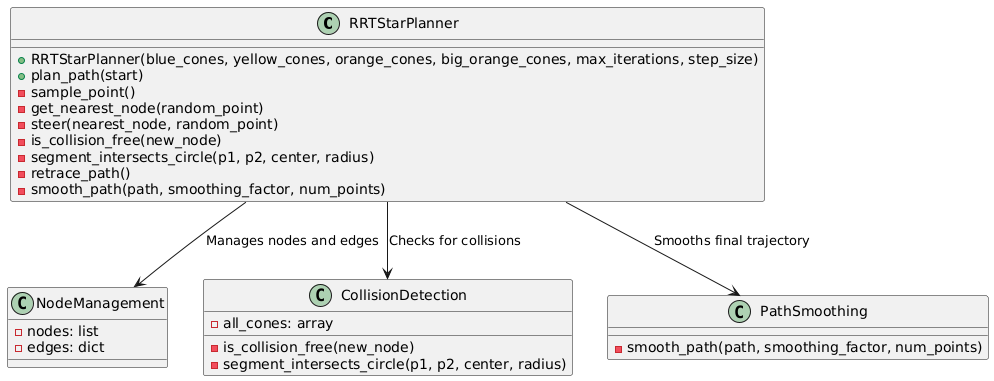
\includegraphics[width=\textwidth]{Images/rrt.png}
    \caption{RRT* Path Planning Structure}
    \label{fig:rrtstar_structure}
\end{figure}

RRT* was chosen due to its ability to generate adaptive paths in dynamic environments while ensuring path optimization over iterations. The planner consists of key modules that handle node expansion, collision avoidance, and final path smoothing.

\subsection{RRT vs. RRT*: Key Differences}

Although both RRT (Rapidly-exploring Random Tree) and RRT* (RRT Star) belong to the same family of sampling-based path planning algorithms, they serve different purposes when applied to real-world autonomous systems. RRT is designed to quickly find any feasible path from a start to a goal state. It is computationally efficient and particularly useful in high-dimensional configuration spaces. However, it does not guarantee path optimality, often producing jagged or unnecessarily long routes. In contrast, RRT* extends RRT by continuously rewiring the tree during expansion, gradually optimizing the path length and smoothness.

In the context of our autonomous racing vehicle, optimality and continuity are not just desired—they are essential. The OBRA car operates in a constrained and dynamic workspace defined by cones that may vary in density, spacing, and even presence due to sensor limitations. In such conditions, simply finding a valid path, as RRT does, is insufficient. We require paths that are not only collision-free but also minimize sharp steering inputs, maximize smoothness, and stay close to the racing line to reduce lap time.

RRT* addresses these requirements directly. By incrementally improving the path as new nodes are added, it creates trajectories that are smoother and more centered. This reduces mechanical stress on the car's steering system and increases overall stability, especially in high-speed sections or tight turns. Furthermore, the ability of RRT* to adapt to local changes in the environment makes it more robust for real-time racing, where missing cones or sudden layout shifts may occur. 

Although RRT* incurs a slightly higher computational cost due to its optimization phase, we mitigated this by carefully tuning key parameters such as step size and maximum iterations. The result is a planner that operates within the real-time constraints of our onboard system while producing higher-quality paths than its predecessor. For this reason, RRT* was selected as the foundation for our planner, offering a balance between flexibility, efficiency, and trajectory quality that aligns with the specific demands of the OBRA car and the racing domain.


\subsection{Initial RRT* Planner: Centerline Trajectory}

In order to perform a meaningful comparison between the RRT* planner and the existing Delaunay-based planner, the first version of RRT* was designed to follow a trajectory biased toward the center of the track. This decision was motivated by the behavior of the Delaunay planner, which inherently produces paths that pass through the midpoints of adjacent cones. Therefore, centering the initial RRT* implementation enables a direct evaluation in terms of smoothness, adaptability, and precision under similar constraints.

To achieve this central bias, the sampling function \texttt{sample\_point()} was engineered to generate random points with a preference for the geometric center between blue and yellow cones. This is implemented by calculating the average position of cones on both sides of the track and biasing new random points toward that mean:

\begin{verbatim}
track_center_x = (np.mean(self.blue_cones[:, 0]) + np.mean(self.yellow_cones[:, 0])) / 2
track_center_y = (np.mean(self.blue_cones[:, 1]) + np.mean(self.yellow_cones[:, 1])) / 2
track_center = np.array([track_center_x, track_center_y])
...
random_point = random_point * (1 - bias_factor) + track_center * bias_factor
\end{verbatim}

A \texttt{bias\_factor} of 0.2 ensures that, while points retain some randomness to enable exploration, they are gently pulled toward the central path. Additionally, a slight outward shift is applied to increase spacing from the cones and reduce the risk of near-collisions:

\begin{verbatim}
shift_distance = 1.2
random_point += shift_distance * (random_point - track_center) / np.linalg.norm(random_point - track_center)
\end{verbatim}

As a result, the generated tree grows in a way that naturally follows the middle of the corridor defined by the cones, producing paths that are smoother and more aligned with the behavior of the Delaunay planner. This configuration is essential for isolating the specific benefits of RRT*, such as adaptability to missing cones or sharper turns, without introducing bias due to fundamentally different target trajectories.

Future versions of the planner, discussed in the next section, will explore more aggressive strategies focused on minimizing lap time rather than maintaining central alignment.


\subsubsection{Node Expansion and Distance Selection}
The RRT* planner expands nodes in the direction of randomly sampled points to explore the space efficiently. The step size is set to \textbf{5 units} to balance coverage and computational efficiency:

\begin{verbatim}
def steer(self, nearest_node, random_point):
    """
    Generates a new node in the direction of `random_point`, limited by `step_size`.
    """
    direction = (random_point - nearest_node) / np.linalg.norm(random_point - nearest_node)
    new_node = nearest_node + direction * self.step_size
    return new_node
\end{verbatim}

Increasing the number of nodes significantly improves path resolution but also introduces computational overhead. If too many nodes are generated per iteration, the planner overloads the CPU, leading to a \textbf{delayed response} from the car. This delay causes the vehicle to react too late, making it difficult to follow the planned trajectory, ultimately leading to deviations from the track. Through empirical testing, a balance was found where \textbf{25 iterations} provide a good trade-off between accuracy and real-time performance.

\subsubsection{Collision Detection and Safety Constraints}
To ensure the vehicle avoids obstacles, a collision-checking mechanism was implemented. Each new node is validated against the detected cones to ensure a \textbf{safe clearance distance} of at least \textbf{2.5 units}:

\begin{verbatim}
def is_collision_free(self, new_node):
    """
    Returns `True` if `new_node` does not collide with any cone.
    """
    safe_distance = 2.5  # Min clearance from cones
    distances = np.linalg.norm(self.all_cones - new_node, axis=1)
    return np.all(distances > safe_distance)
\end{verbatim}

By maintaining a safe distance from cones, the planner prevents situations where the vehicle may clip obstacles due to minor inaccuracies in perception.

\subsubsection{Path Retracing and Smoothing}
Once a set of valid nodes has been generated, the planner reconstructs the path from the last node back to the start using a retracing mechanism:

\begin{verbatim}
def retrace_path(self):
    """
    Reconstructs the path from the last node to the start.
    """
    last_node = self.nodes[-1]
    path = [last_node]
    while tuple(path[-1]) in self.edges:
        path.append(self.edges[tuple(path[-1])])
    path.reverse()
    return np.array(path)
\end{verbatim}

To further refine the trajectory, a \textbf{spline-based smoothing algorithm} is applied. This ensures the path is continuous and minimizes abrupt steering changes:

\begin{verbatim}
def smooth_path(self, path, smoothing_factor=0.5, num_points=50):
    """
    Uses spline interpolation to generate a smoother trajectory.
    """
    tck, u = splprep([path[:, 0], path[:, 1]], s=smoothing_factor, k=min(3, len(path)-1))  
    x_smooth, y_smooth = splev(np.linspace(0, 1, num_points), tck)
    return np.vstack((x_smooth, y_smooth)).T
\end{verbatim}

Smoothing eliminates unnecessary oscillations in the path, reducing the load on the vehicle's steering system and improving driving stability.


\subsection{Final RRT* Planner: Fastest Trajectory}

This version of the RRT* planner is considered the final and most optimal implementation for the OBRA car, as it is explicitly designed to follow the fastest possible trajectory through the track rather than simply maintaining a central line. While the initial RRT* was biased toward the center to enable direct comparison with the Delaunay planner, this version prioritizes performance, speed, and aggressive maneuvering—factors critical in a competitive racing environment.

The core difference lies in the sampling strategy. Instead of sampling points biased toward the geometric center of the track, this planner favors points further ahead along the driving axis (positive X-direction), encouraging the vehicle to progress rapidly while minimizing lateral deviation. This is reflected in the following line within the \texttt{sample\_point()} method:

\begin{verbatim}
rand_x = np.random.uniform(5, 10)  # Prioritize forward sampling
rand_y = np.random.uniform(-3, 3)  # Allow lateral flexibility
random_point = np.array([car_x + rand_x, car_y + rand_y])
\end{verbatim}

To further enhance safety and maintain aggressive yet reliable driving, sampled points are rejected if they fall too close to any cone:

\begin{verbatim}
distances = np.linalg.norm(self.all_cones - random_point, axis=1)
if np.any(distances < 2.5):
    return self.sample_point()
\end{verbatim}

This ensures that the trajectory not only favors speed but also remains within safe operational margins.

Additionally, this version uses an alignment-weighted nearest node search that prioritizes expansion in the forward direction (X-axis), reinforcing the planner’s bias toward the racing line and avoiding backward or inefficient detours:

\begin{verbatim}
goal_direction = np.array([1, 0])  # Favors forward motion
\end{verbatim}

Compared to the initial centerline-focused RRT*, this implementation results in more aggressive paths that cut closer to the apex of turns and reduce total lap distance, while still respecting safety constraints. It is therefore better aligned with the real-world demands of autonomous racing, where maximizing performance per lap is more important than symmetrical navigation.

This final RRT* planner lays the foundation for deployment in the real vehicle, offering a robust balance between real-time feasibility, adaptability, and competitive performance.

\subsection{Final Considerations}

Throughout this project, four distinct path planners were developed and evaluated to explore the trade-offs between stability, adaptability, and performance in autonomous racing: the initial unoptimized Delaunay planner, the improved Delaunay version, a centerline-biased RRT* planner, and the final optimized RRT* for fastest trajectory.

The initial Delaunay planner was the first implemented solution. Although functional, it lacked the flexibility to handle dynamic track variations. It followed a fixed triangulation logic between cones, often generating stable but suboptimal paths. Its limitations became evident when cones were missing, misplaced, or when sharp turns required more dynamic trajectory adaptation.

The optimized Delaunay version addressed some of these issues by refining the triangulation logic, improving midpoint selection, and adjusting parameters to make the output path more consistent. However, it still suffered from structural rigidity, as its connectivity remained dependent on the presence and layout of detected cones. Despite offering better stability than the original version, its adaptability and response time to sudden track changes remained limited.

To overcome these constraints, the RRT* family of planners was introduced. The first implementation was intentionally biased toward the centerline to mirror the typical behavior of the Delaunay planner. This allowed a fair comparison in terms of precision, smoothness, and structural differences. It demonstrated improved handling of irregularities in cone placement, as well as more consistent collision avoidance.

The final and most performant version is the optimized RRT* planner targeting the fastest possible trajectory. Unlike its predecessors, it no longer follows a geometric centerline but actively searches for paths that minimize total driving distance and improve lap time. Through strategic forward sampling, directionally weighted node expansion, and active cone avoidance, it generates more aggressive and efficient routes. While this introduces higher computational complexity, the parameters were carefully tuned to maintain real-time performance on the OBRA car's onboard system.

In summary, the planners form a clear progression:
\begin{itemize}
    \item \textbf{Initial Delaunay}: Basic, stable, but limited and rigid.
    \item \textbf{Optimized Delaunay}: More stable and refined, yet still constrained by static structure.
    \item \textbf{Centerline RRT*}: Flexible and robust, ideal for comparison and mid-level adaptation.
    \item \textbf{Final RRT* (Fastest)}: Optimal in performance, adaptable to real-time racing scenarios, and designed for deployment.
\end{itemize}

It is expected that the final RRT* planner will significantly outperform the others in dynamic conditions, especially on sharp turns and incomplete cone layouts. Its adaptive nature and path optimization capabilities make it the most promising solution for real-world autonomous racing.

\newpage


\chapter {Version Management}

\section{Source Code and Data Management}

Version control plays a crucial role in the development of this project, ensuring efficient collaboration, structured code management, and reliable tracking of modifications. For this purpose, we utilize Git alongside GitLab, where the OBRA team's centralized workspace is hosted. GitLab serves as the primary repository, storing all project files, code implementations, and historical data from previous years.

At the beginning of the project, the entire existing workspace was cloned from GitLab, providing access to all prior developments, including path-planning algorithms and other essential components used by the team in past seasons. This initial setup allowed us to build upon a solid foundation while ensuring compatibility with the existing autonomous system. Throughout the development process, every modification and improvement to the path planners has been systematically managed using branches within our GitLab repository. Each time a new version of a path-planning algorithm was implemented—whether modifications to the Delaunay planner or the development of the RRT/RRT* algorithm—a dedicated branch was created. This approach enabled parallel development and testing of different versions while preserving the stability of the main codebase.

To maintain an organized and up-to-date repository, commits have been made regularly, ensuring that every iteration and refinement is properly documented. This frequent commit practice has allowed us to track changes efficiently, revert to previous versions when necessary, and collaborate seamlessly within the team. By leveraging GitLab's version control features, we have established a structured workflow that facilitates code reviews, debugging, and continuous integration, ultimately enhancing the reliability of our path-planning system.

In addition to code management, we use Notion to coordinate team tasks and maintain an Agile workflow. Notion enables us to assign responsibilities, track progress, and ensure development efforts remain aligned with project goals. Furthermore, all generated data, including test results, simulation outputs, and performance evaluations, are stored in Google Drive. This provides a centralized location for data accessibility, allowing for efficient documentation and analysis of algorithm performance over time.

\subsection{GitLab Repository Structure (Aquí puedes incluir una imagen del esquema del repositorio)}

\subsection{Source Code Repository Link}
URL or reference to the project repository.

\newpage

\chapter{Results}
\section{Results and Testing}
\subsection{Simulation Setup}
Explanation of the Unity + ROS2 environment configuration.

\subsection{Test Scenarios}
List of simulated scenarios used for validation.

\section{Performance Metrics}
\subsection{Computation Time Evaluation}
Data on execution times.

\subsection{Path Quality Analysis}
Metrics evaluating the efficiency and smoothness of generated paths.

\subsection{Adaptability to Dynamic Obstacles}
Explanation of testing under dynamic conditions.

\section{Experimental Results}
\subsection{Comparison of Metrics Between Optimized Delaunay and RRT*, or all planners}
Presentation of comparative data.

\subsection{Visualization of Results Through Graphs}
Graphs and their interpretation.

\subsection{Code Efficiency and Optimization Metrics}

\newpage

\chapter{Professionalism}
\section{Project Management}
\subsection{Development Activities and Schedule}
Project logs, reports, and Gantt charts.

\subsection{Data Management}
Storage and organization of research documents.

\subsection{Project Deliverables}
Summary of key milestones.

\section{Risk Analysis}
\subsection{Identified Risks and Mitigation Strategies}
Discussion of risks encountered and strategies used.

\subsection{Updated Project Plan Based on Risk Evaluation}
Adjustments made due to identified risks.

\section{Legal, Ethical, and Environmental Considerations}
\subsection{Compliance with Professional Codes of Conduct}
References to BCS, ACM, and industry standards.

\subsection{Ethical and Environmental Impact of the Project}
Analysis of social and environmental implications.

\newpage

\chapter{Conclusion}
\section{Summary of Findings}
\subsection{Key Insights from the Algorithm Comparison}
Main takeaways from testing and evaluation.

\section{Future Work}
\subsection{Improvements in RRT* Implementation}
Potential refinements to enhance algorithm performance.

\subsection{Real-World Applications}
Application of findings to actual autonomous vehicle scenarios.

\newpage

\chapter{Bibliography}
\bibliographystyle{IEEEtran}
\begin{thebibliography}{4}

    \bibitem{reference1} LaValle, S. (2006) 'Rapidly exploring Random Trees: Overview', Available at: \url{https://lavalle.pl/rrt} (Accessed: 10 October 2024).
    
    \bibitem{reference2} Bécsi, T. (2024) 'RRT-guided experience generation for reinforcement learning in autonomous lane keeping', Scientific Reports, 14, Article number: 24059. Available at: \url{https://www.nature.com/articles/s41598-024-73881-z} (Accessed: 16 October 2024).
    
    \bibitem{reference3} Muhsen, D.K., Raheem, F.A., and Sadiq, A.T. (2024) 'A Systematic Review of Rapidly Exploring Random Tree RRT Algorithm for Single and Multiple Robots', Cybernetics and Information Technologies, 24(3), pp. 78-101. Available at: \url{https://doi.org/10.2478/cait-2024-0026} (Accessed: 19 September 2024).
    
    \bibitem{reference4} Fan, H., Huang, J., Huang, X., Zhu, H., and Su, H. (2024) 'BI-RRT*: An improved path planning algorithm for secure and trustworthy mobile robots systems', Heliyon, 24(e26403). Available at: \url{https://doi.org/10.1016/j.heliyon.2024.e26403} (Accessed: 10 October 2024).
    
\end{thebibliography}

\newpage
 
\chapter{Appendices}
\section{Supplementary Data}
\subsection{Source Code Repository (GitHub/GitLab)}
Reference link to the source code.

\subsection{ROS2 + Unity Configuration Details}
Technical setup instructions.

\subsection{Raw Simulation Results}
Unprocessed data from testing and evaluation.

\end{document}
